\section{Statistical model for fit to data}
\label{sec:htoinv_satistical_treatment}

A likelihood model is used in the fit to data, simultaneously over the signal and \glspl{CR} to obtain the \acrlong{sm} expectation values as well as testing for signals of the \higgstoinv decay. Events are categorised in two dimensions: the subcategories that target specific Higgs boson production modes and final state topologies as per Tab.~\ref{tab:htoinv_categories}, and in bins of \ptmiss as per Chpt.~\ref{subsec:htoinv_binning}. The observed event counts from data in each subcategory and \ptmiss bin are modelled as Poisson-distributed variables around the \acrshort{sm} expectation with a potential contribution from signal (assumed to be zero in the null hypothesis). Expected event counts in the signal region are obtained from simulation, aided by predictions from the \glspl{CR} and \glspl{SB} for non-multijet and \acrshort{qcd} multijet processes, respectively. These are elaborated upon in Chpt.~\ref{subsec:htoinv_background_est}. Systematic uncertainties associated with the non-multijet processes, discussed in Chpt.~\ref{sec:htoinv_mc_corrections}, are incorporated as nuisance parameters within the model. The likelihood function $\likelihood_{\higgstoinv}$ can be summarised as
\begin{equation}
    \likelihood_{\higgstoinv} = \likelihood_{\mathrm{SR}} \cdot \likelihood_{\text{\singleMuCr CR}} \cdot \likelihood_{\text{\doubleMuCr CR}} \cdot \likelihood_{\text{\singleEleCr CR}} \cdot \likelihood_{\text{\doubleMuCr CR}} \cdot \likelihood_{\text{\singlePhotonCr CR}}
    \label{eq:likelihood_overall}
\end{equation}

where the aim of the fit is to minimise $-\ln \likelihood_{\higgstoinv}$. The likelihood in a given region of the analysis may be written as multiple Poisson likelihoods, denoting $\mathcal{P}(n | \lambda) \equiv \frac{ e^{-\lambda} \lambda^n }{n!}$. In the signal region,
\begin{equation}
    \begin{aligned}
\likelihood_{\mathrm{SR}}(r, a_{\lostlepton}, a_{\ztonunu}, \rho) &= \prod_{i} \prod_{j(i)} \mathcal{P}(N_{\mathrm{obs.}}^{i, j} | N_{\mathrm{pred.}}^{i, j}), \ \text{where}\\
N_{\mathrm{pred.}}^{i, j} &= r \cdot s^{i, j} \cdot \rho_s^{i, j}\\
&+ b_{\lostlepton}^{i, j} \cdot a_{\lostlepton}^{i, j} \cdot \rho_{\lostlepton}^{i, j}\\
&+ b_{\ztonunu}^{i, j} \cdot a_{\ztonunu}^{i, j} \cdot \rho_{\ztonunu}^{i, j}\\
&+ c_{\mathrm{QCD}}^{i, j} \cdot \omega_{\mathrm{QCD}}^{i, j}
    \end{aligned}
    \label{eq:likelihood_SR}
\end{equation}

where the indices $i$ and $j$ refer to each subcategory and \ptmiss bin, respectively, $r$ is the unconstrained signal strength parameter, i.e., \BRHinvFull, $s$ is the signal expectation determined from simulation, $\rho$ encodes the systematic uncertainties associated with simulation, $b$ is the number of events from simulation, $a$ is an unconstrained rate parameter connecting the signal and corresponding \glspl{CR}, $c$ is the predicted number of events, and $\omega$ contains the uncertainties on the \acrshort{qcd} multijet background estimate. Similarly for the control regions, the likelihood functions are
\begin{equation}
    \begin{aligned}
\likelihood_{\text{\singleMuCr CR}} &= \prod_{i} \prod_{j(i)} \mathcal{P}( N_{\mathrm{obs.}, \, \Pmu }^{i, j} | r \cdot s^{i, j}_{\Pmu} \cdot \rho_{s,\, \Pmu}^{i, j} + b_{\Pmu}^{i, j} \cdot a_{\lostlepton}^{i, j} \cdot \rho_{\Pmu}^{i, j} )\\
\likelihood_{\text{\doubleMuCr CR}} &= \prod_{i} \prod_{j(i)} \mathcal{P}( N_{\mathrm{obs.}, \, \Pmu\Pmu }^{i, j} | r \cdot s^{i, j}_{\Pmu\Pmu} \cdot \rho_{s,\, \Pmu\Pmu}^{i, j} + b_{\Pmu\Pmu}^{i, j} \cdot a_{\ztonunu}^{i, j} \cdot \rho_{\Pmu\Pmu}^{i, j} )\\
\likelihood_{\text{\singleEleCr CR}} &= \prod_{i} \prod_{j(i)} \mathcal{P}( N_{\mathrm{obs.}, \, \Pe }^{i, j} | r \cdot s^{i, j}_{\Pe} \cdot \rho_{s,\, \Pe}^{i, j} + b_{\Pe}^{i, j} \cdot a_{\lostlepton}^{i, j} \cdot \rho_{\Pe}^{i, j} )\\
\likelihood_{\text{\doubleEleCr CR}} &= \prod_{i} \prod_{j(i)} \mathcal{P}( N_{\mathrm{obs.}, \, \Pe\Pe }^{i, j} | r \cdot s^{i, j}_{\Pe\Pe} \cdot \rho_{s,\, \Pe\Pe}^{i, j} + b_{\Pe\Pe}^{i, j} \cdot a_{\ztonunu}^{i, j} \cdot \rho_{\Pe\Pe}^{i, j} )\\
\likelihood_{\text{\singlePhotonCr CR}} &= \prod_{i} \prod_{j(i)} \mathcal{P}( N_{\mathrm{obs.}, \, \Pphoton }^{i, j} | r \cdot s^{i, j}_{\Pphoton} \cdot \rho_{s,\, \Pphoton}^{i, j} + b_{\Pphoton}^{i, j} \cdot a_{\ztonunu}^{i, j} \cdot \rho_{\Pphoton}^{i, j} + c_{\mathrm{QCD}}^{i, j} \cdot \omega_{\mathrm{QCD}}^{i, j} )
    \end{aligned}
    \label{eq:likelihood_CRs}
\end{equation}

where the products over the indices $i$ and $j$ are the same as in Eq.~\ref{eq:likelihood_SR}. Signal contamination $s$ is accounted for in all \glspl{CR}. The rate parameters $a$ are shared across the complementary \glspl{CR} for the same subcategories and \ptmiss bins, i.e., $a_{\lostlepton}$ in the single lepton regions, and $a_{\ztonunu}$ in the dilepton and single photon regions. \acrshort{qcd} multijet \acrshort{mc} is not included in any of the lepton \glspl{CR}, but is estimated in the \singlePhotonCr \gls{CR} from the photon purity measurement recounted in Chpt.~\ref{subsubsec:htoinv_photon_purity}.

The \CLs method~\cite{Read_2002} for setting an upper limit on $r$ is used in the case no new physics is observed. It is often applied to set exclusion limits on non-negative parameters. Instead of simply comparing the $p$-value from the signal plus background (alternative) hypothesis $p_{s+b}$---obtained from the fit---to the threshold $\alpha$, both $p_{s+b}$ and the $p$-value from the background-only (null) hypothesis $p_b$ are involved. The alternative hypothesis is rejected, i.e., the signal model is excluded, where
\begin{equation}
    \frac{p_{s+b}}{1 - p_b} \leq \alpha
    \label{eq:CLs_ratio}
\end{equation}

As such, the upper limit on the signal strength parameter is given by the value of $r$ in which the left-hand side of Eq.~\ref{eq:CLs_ratio} equals $\alpha$. An asymptotic formula~\cite{Cowan:2010js}, whereby the ensemble of simulated datasets is replaced the single, representative one to reduce computational expense, is applicable in the large sample limit and is incorporated into the model.

Statistical uncertainties from simulation are accommodated as a single nuisance parameter per bin based on Ref.~\citenum{BARLOW1993219}. Above 10 weighted events, the uncertainty is profiled according to a Gaussian distribution centred on its value. Below that threshold, a Poisson distribution is instead invoked to provide stability in the fit for bins with small event counts. These methods are implemented, along with the likelihood function, in the \textsf{HiggsAnalysis-CombinedLimit} package.

% Current fit model is given at https://indico.cern.ch/event/934008/contributions/3924639/attachments/2065231/3465892/2020_06_15_CHIP_Meeting_nonVBF_fit.pdf

% Toys (verbatim from Henning): toys are repeat experiments where you draw new values for your observed signal and background based on the uncertainties associated with both. The parameters values are randomly drawn according to some pdf. I.e. if we talk about large event counts this would be gaussian with width equal to uncertainty,  small event counts Poissonian, for syst uncert possibly log-normal.


%=========================================================


\subsection{Binning}
\label{subsec:htoinv_binning}

In addition to the categories in Chpt.~\ref{sec:htoinv_categorisation}, events are further separated into bins of \ptmiss as that distribution is expected to maximally differentiate signal and background in the fit. Since the number of events can significantly differ between categories in the different regions of the analysis, a global binning configuration is inadequate. For each subcategory, the number and widths of the bins are tuned to ensure sufficient statistical precision. These schemes are tied to the subcategory, so are reflected in all regions such that the background estimation methods can operate on a bin-by-bin basis. The binning configuration is outlined in Tab.~\ref{tab:htoinv_binning_scheme}.

\begin{table}[htbp]
    \centering
    \begin{tabular}{ccl}
        \hline\hline
        Category & Subcategory & \ptmiss bins (GeV) \\\hline
        \multirow{9}{*}{\ttH} & 2Boosted & [200, 300), [300, 400), [400, $\infty$) \\
        & 1t1b & [200, 300), [300, 400), [400, $\infty$) \\
        & 1t2b & [200, 300), [300, 400), [400, 600), [600, $\infty$) \\
        & 1W1b & [200, 300), [300, 400), [400, $\infty$) \\
        & 1W2b & [200, 300), [300, 400), [400, $\infty$) \\
        & 5j1b & [200, 300), [300, 400), [400, $\infty$) \\
        & 6j1b & [200, 300), [300, 400), [400, $\infty$) \\
        & 5j2b & [200, 300), [300, 400), [400, $\infty$) \\
        & 6j2b & [200, 300), [300, 400), [400, $\infty$) \\\hline
        \multirow{4}{*}{\VH} & 2j0b & [200, 300), [300, 400), [400, $\infty$) \\
        & 2j1b & [200, 300), [300, 400), [400, $\infty$) \\
        & 2j2b & [200, $\infty$)\\
        & 1V & [200, 300), [300, 400), [400, $\infty$) \\\hline
        \multirow{4}{*}{\ggH}& 2jM & [200, 300), [300, 400), [400, 600), [600, 900), [900, $\infty$) \\
        & 3j & [200, 300), [300, 400), [400, 600), [600, 900), [900, $\infty$) \\
        & 4j & [200, 300), [300, 400), [400, 600), [600, 900), [900, $\infty$) \\
        & 5j & [200, 300), [300, 400), [400, 600), [600, 900), [900, $\infty$) \\
        \hline\hline
    \end{tabular}
    \caption[The binning scheme used to categorise events in terms of \ptmiss]{The binning scheme used to categorise events in terms of \ptmiss.}
    \label{tab:htoinv_binning_scheme}
\end{table}


%=========================================================


\subsection{Background estimation}
\label{subsec:htoinv_background_est}

Accurate estimation of the \acrlong{sm} background processes in the signal region is paramount to a search for new physics. Mismeasured backgrounds and uncertainties can wash out traces of signal and affect the fit to data. In the signal region and \acrshort{qcd} sidebands, simulated samples in Chpt.~\ref{subsec:htoinv_background} are grouped into three processes for the purposes of background estimation in the fit:

\medskip

\begin{easylist}[itemize]
    \easylistprops
    & Lost lepton: Comprised of electroweak $\PW + \text{2 jets}$, \gammapjets, single top, \ttbarpjets, $\ttbar\Pphoton \plusjets$, $\ttbar\PW \plusjets$, $\ttbar\PH \plusjets$, and \wtolnupjets
    & $\ztonunu$: Comprised of Drell-Yan $(\HepProcess{\PZ \to \Plepton\Plepton}) \plusjets$, multiboson, electroweak $\PZ + \text{2 jets}$, $\ttbar\PZ \plusjets$, and \ztonunupjets
    & \acrshort{qcd}: \acrshort{qcd} multijet
\end{easylist}

\medskip

\noindent{}In the lepton \glspl{CR}, all samples are grouped into a single ``electroweak'' process with the exception of \acrshort{qcd} multijet that is absent entirely. In the \singlePhotonCr \gls{CR}, the non-multijet datasets are also under the electroweak label, and the presence of \acrshort{qcd} is estimated from the photon purity measurement.

The single lepton \glspl{CR} are used to constrain the lost lepton background in the signal region, arising primarily from \ttbarpjets and \wtolnupjets. The dilepton and photon \glspl{CR} predict the \ztonunupjets background. These estimations rely on the data and \acrlong{mc} yields in those regions, controlled via a rate parameter to connect them to the signal region. \Glspl{SB} to the signal region estimate \acrshort{qcd} multijet contributions from data. The prediction in this case takes the form of a \emph{transfer factor} method---a constrained application of a rate parameter. Prediction of the background yields from each of these methods is done so within the fit and expressed in the likelihoods. Further explanation is given below. Fig.~\ref{fig:htoinv_fit_overview} illustrates the correspondence between the analysis regions and background predictions.

\begin{figure}[htbp]
    \centering
    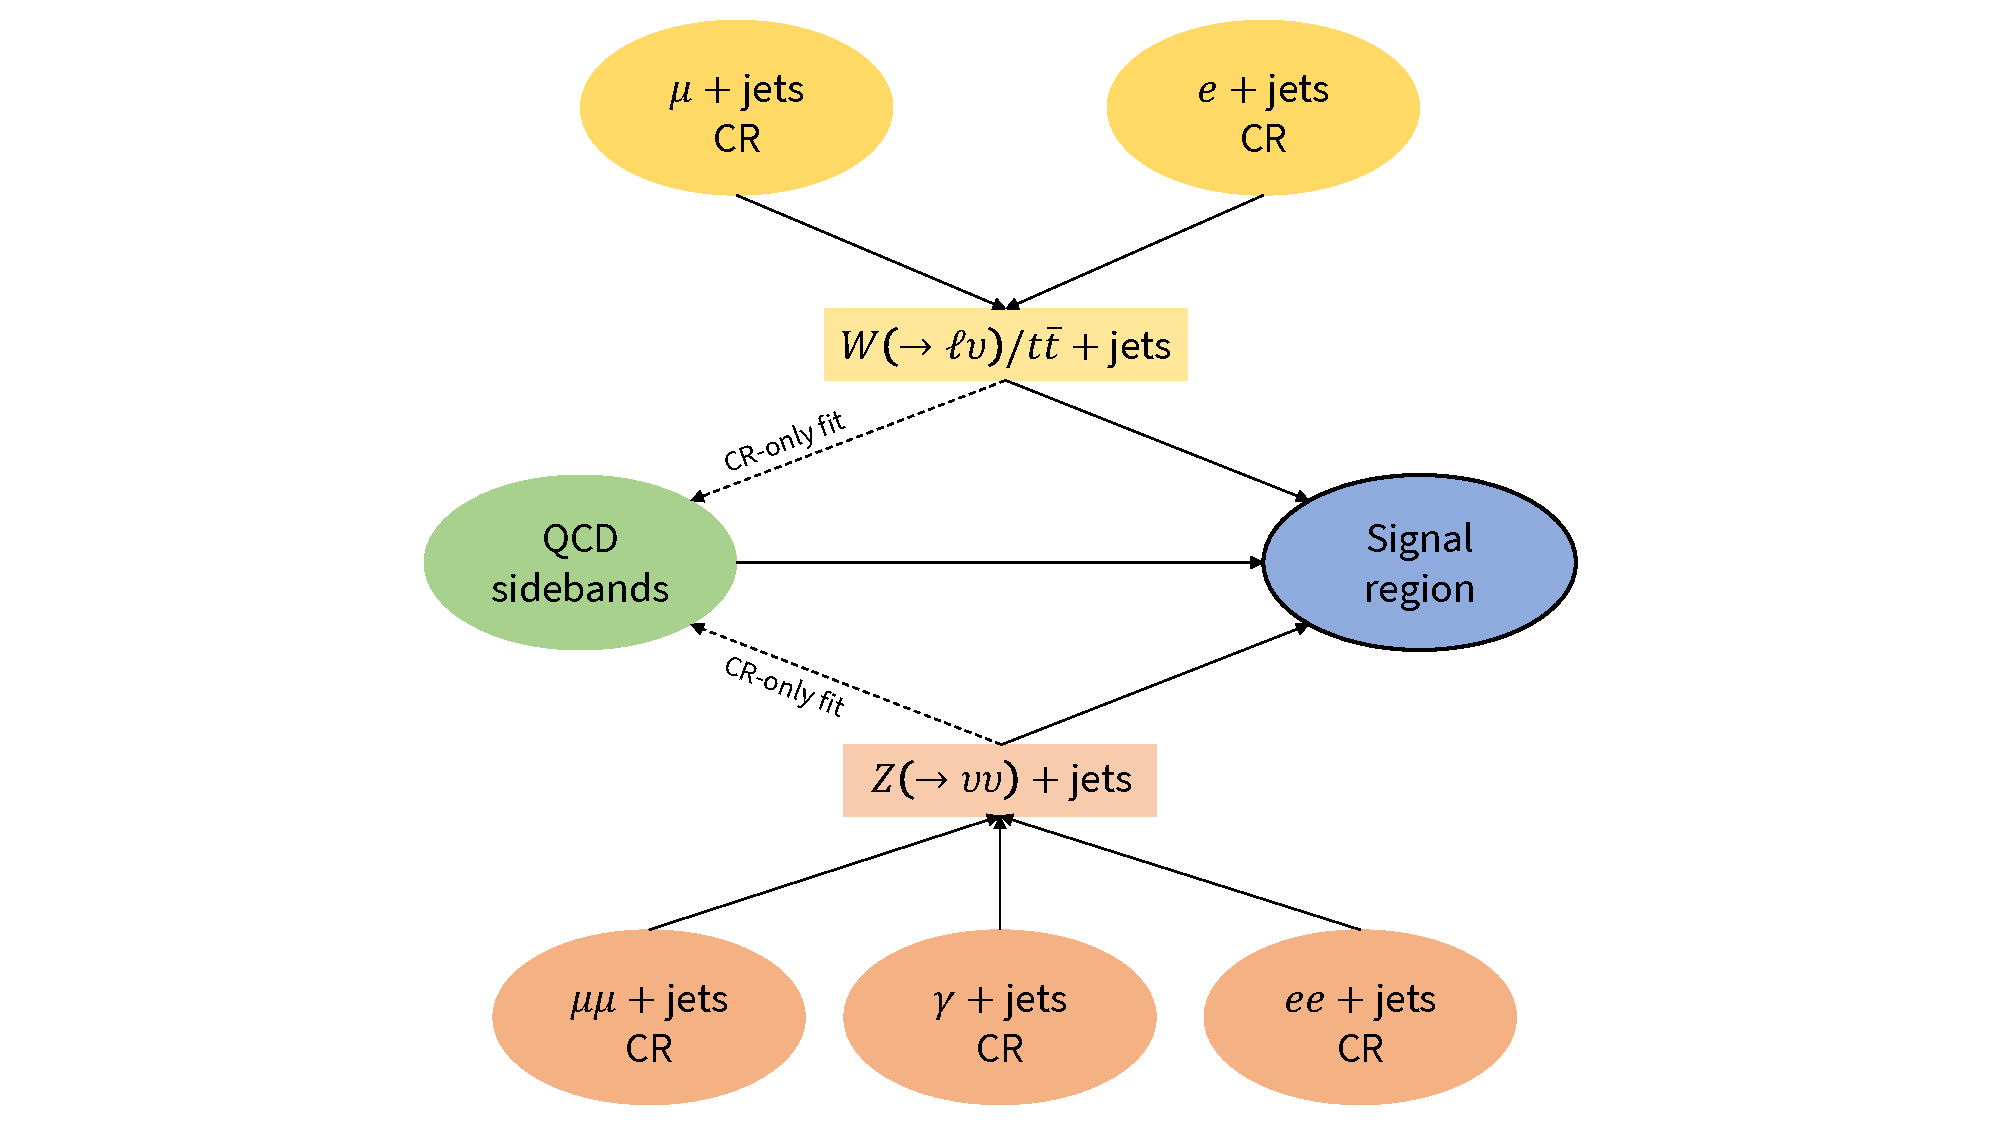
\includegraphics[width=0.5\textwidth]{figures/fit_overview.pdf}
    \caption[An infographic showcasing the role of each analysis region in the final fit]{An infographic showcasing the role of each analysis region in the final fit. The \glspl{CR} predict the lost lepton and \ztonunu backgrounds, and a \gls{CR}-only fit informs the \acrshort{qcd} multijet prediction that contributes to the eventual background determination in the signal region.}
    \label{fig:htoinv_fit_overview}
\end{figure}


%=========================================================


\subsubsection{Lost lepton (\texorpdfstring{$\mkern-2mu\PW$}{W} and \texorpdfstring{$\ttbarpjets$}{ttbar plus jets})}
\label{subsubsec:htoinv_lost_lepton_bkg}

In order to predict the lost lepton background in the signal region, a freely floating rate parameter $a_{\lostlepton}$ is introduced in the fit. It is shared across the single lepton \glspl{CR} and signal region, where it scales the event count from simulation in these regions to obtain the expected values. Events are categorised and binned in the same manner in the single lepton \glspl{CR} as in the signal region, such that the rate parameters---and therefore the prediction---is derived bin-by-bin. The predicted number of lost lepton events in Eqs.~\ref{eq:likelihood_SR} and \ref{eq:likelihood_CRs} is then simply $b_{\lostlepton} \cdot a_{\lostlepton}$.


%=========================================================


\subsubsection{\texorpdfstring{\ztonunupjets}{Z to nunu + jets}}
\label{subsubsec:htoinv_znunu_bkg}

The irreducible background from invisibly decaying \PZ bosons is estimated in the same manner as the lost lepton background. A rate parameter $a_{\ztonunu}$ ties together the dilepton \glspl{CR}, the photon \gls{CR}, and the signal region. The yields from simulation are scaled by the best fit value of the parameter, obtained during the simultaneous fit to the analysis regions. As with the lost lepton background, event categorisation is the same in these regions, allowing the predictions to be derived independently for each subcategory and \ptmiss bin. 


%=========================================================


\subsubsection{QCD multijet}
\label{subsubsec:htoinv_qcd_multijet_bkg}

The effects of \gls{jet} mismeasurements are difficult to quantify. With a final state of several \glspl{jet} in the \acrshort{qcd} multijet process, low, or even no, \ptvecmiss is expected. Therefore, a single mismeasured \gls{jet} will introduce artificial \ptvecmiss in the direction of that jet. A low $\mindphiAB{\mathrm{j}}{\ptvecmiss}$ is therefore expected. Though it is not just this process that suffers---\glspl{jet} from ``cleaner'' processes may also be affected---those with real \ptmiss in an event (e.g., $\ztonunupjets$) are unlikely to be significantly affected by one stray object. The enormous cross section of \acrshort{qcd} multijet also amplifies the problem, making the process as a whole more sensitive to, e.g., fluctuations in the calorimeter response that would affect the energy measurement.

Contributions to the signal region from \acrshort{qcd} multijet events should be adequately suppressed by the analysis-level selection requirements. However, it is still a process that must be accurately accounted for considering its rate of production at \acrshort{cms}. A metric by which to estimate the number of events a dataset should require is by calculating the equivalent luminosity:
\begin{equation}
    \lumi_{\mathrm{eq.}} = \frac{N_{\mathrm{events}}}{\sigma}
    \label{eq:equivalent_lumi}
\end{equation}

A general rule is that the equivalent luminosity of a given dataset should be comparable to, or even exceed, that of the data collected by the experiment. Since the \acrshort{qcd} multijet process has a very large cross section, simulating the required number of events to match the luminosity of the data recorded during Run-2 is not feasible. This can be mitigated by using a data-driven method to estimate it from the multijet-enriched sidebands described in Chpt.~\ref{subsec:htoinv_sidebands}.

To estimate the presence of \acrshort{qcd} in the signal region, a data driven approach is taken utilising the sidebands defined in Chpt.~\ref{subsec:htoinv_sidebands}. These are derived separately for each category and data taking year. Firstly, a fit using the \glspl{CR} is performed to extract the rate parameters ($a$ from Eq.~\ref{eq:likelihood_CRs}) that scale the non-multijet background in each subcategory and \ptmiss bin. Applying these to the corresponding backgrounds in the sidebands changes the event distribution and hence the data/\acrshort{mc} agreement. The excess in data in a sideband is assumed to arise solely from multijet events, and as such the difference between data and the non-multijet background is attributed to \acrshort{qcd} (denoted as $N_{\mathrm{SB}}^{\mathrm{QCD}}$).

\acrshort{qcd} in the signal region $N_{\mathrm{pred.}}^{\mathrm{QCD}}$ (corresponding to $c_{\mathrm{QCD}}$ in Eq.~\ref{eq:likelihood_SR}) is predicted in each subcategory and \ptmiss bin as follows: 
\begin{equation}
    N_{\mathrm{pred.}}^{\mathrm{QCD}}(\text{subcategory}, \, \ptmiss) = N_{\mathrm{SB}}^{\mathrm{QCD}} \cdot \transfac_{\mathrm{QCD}} \cdot \catFraction(\text{subcategory}) \cdot \metFraction(\ptmiss)
    \label{eq:qcd_prediction}
\end{equation}

where $\transfac_{\mathrm{QCD}}$ is the transfer factor relating the \acrshort{qcd} in the sideband to the multijet simulation in the signal region. As the signal region is depleted in simulated multijet events, the transfer factor is inclusive over the region rather than per \ptmiss bin and subcategory, i.e.,
\begin{equation}
    \transfac_{\mathrm{QCD}} = \frac{ N_{\mathrm{MC, \ SR}}^{\mathrm{QCD}} } { N_{\mathrm{MC, \ SB}}^{\mathrm{QCD}} }
%   \transfac_{\mathrm{QCD}} = \frac{ \sum_{\text{subcategory}, \, \ptmiss}^{\mathrm{SR}} N_{\mathrm{MC}}^{\mathrm{QCD}}(\text{subcategory}, \, \ptmiss) }{ \sum_{\text{subcategory}, \, \ptmiss}^{\mathrm{SB}} N_{\mathrm{MC}}^{\mathrm{QCD}}(\text{subcategory}, \, \ptmiss) }
    \label{eq:transfer_factor_qcd}
\end{equation}

% To mitigate the statistical limitations of the \acrshort{qcd} \acrshort{mc} nominally used in the analysis, to determine the transfer factor, their event count was increased a hundredfold using a ``smear and rebalance'' method as performed in Ref.~\citenum{Sirunyan:2017wif}.
The distribution of the \acrshort{qcd} background for each subcategory and \ptmiss bin is extrapolated from the sidebands with the factors $\catFraction$ and $\metFraction$. $\catFraction$ is the fraction of non-\acrshort{qcd} \acrshort{mc} in a given subcategory of a given sideband, inclusive of \ptmiss. $\metFraction$ is the fraction of non-\acrshort{qcd} \acrshort{mc} in a given \ptmiss bin of a given sideband, inclusive of subcategory. Even in the multijet enriched sidebands, particularly for the \ttH category, low yields of \acrshort{qcd} \acrshort{mc} are seen and subject to statistical fluctuations. Determining $\catFraction$ and $\metFraction$ from non-multijet simulation assumes the \acrshort{qcd} background is distributed in the same proportion across subcategories as the the non-\acrshort{qcd} background, though gives a more consistent description of the data in the sidebands than estimating the fractions from \acrshort{qcd} \acrshort{mc}. A 50\,\% uncertainty following a log normal distribution is assigned to the predicted multijet event counts.
